\documentclass[10pt,letterpaper]{article}
\usepackage[margin=0.66in,top=0.60in,bottom=0.61in]{geometry}
\usepackage[T1]{fontenc}
\usepackage{lmodern,microtype,amsmath,amssymb,booktabs,array,graphicx,xcolor}
\usepackage{fancyhdr,enumitem,hyperref,url}
\definecolor{ink}{HTML}{153C51}
\definecolor{muted}{HTML}{53636D}
\hypersetup{colorlinks=true,urlcolor=ink,linkcolor=ink,pdftitle={2021 conditional upper-limit echoes: v5.6.1},pdfauthor={Emrys Peets}}
\setlength{\parindent}{0pt}\setlength{\parskip}{5pt}
\setlength{\emergencystretch}{1em}
\setlength{\headheight}{13pt}\setlength{\headsep}{10pt}\setlength{\footskip}{18pt}
\addtolength{\topmargin}{8pt}\addtolength{\textheight}{-8pt}
\setlength{\tabcolsep}{4.5pt}\renewcommand{\arraystretch}{1.11}
\pagestyle{fancy}\fancyhf{}
\fancyhead[L]{\small\color{muted}HPS GPR \quad 2021 upper-limit echoes}
\fancyhead[R]{\small\color{muted}v5.6.1}
\fancyfoot[L]{\footnotesize\color{muted}Conditional simulated full-statistics catalogue}
\fancyfoot[R]{\footnotesize\thepage}
\renewcommand{\headrulewidth}{0.25pt}
\newcommand{\heading}[1]{\vspace{2pt}{\Large\bfseries\color{ink}#1}\par\vspace{3pt}}
\newcommand{\subheading}[1]{\par\vspace{4pt}{\bfseries\color{ink}#1}\par}
\newcommand{\smallnote}[1]{{\small\color{muted}#1}\par}
\newcommand{\nextpage}{\clearpage}
\begin{document}

{\small\color{muted}13 September 2026 \hfill Extension of the v5.6 peak catalogue}\par
\vspace{6pt}
{\LARGE\bfseries\color{ink}Conditional upper-limit echoes\\[3pt]from projected 2021 peaks}\par
\vspace{5pt}
This extension follows the v5.6 injected peaks across the mass scan to predict
nearby upper-limit dips, or \emph{echoes}. It reuses all 300 saved toys across
15 scenarios, with separate nominal $1\%\times100$ and $10\%\times10$ projections.

\subheading{The local-significance scaling that motivates the injections}
For unchanged selection and shapes, a persistent excess dominated by counting
statistics scales with the exposure multiplier $k=1/f$ as
\begin{equation}
\begin{gathered}
 S_{100\%}=kS_f,\qquad B_{100\%}=kB_f,\qquad
 Z_{100\%}\simeq\frac{kS_f}{\sqrt{kB_f}}=\sqrt{k}\,Z_f,\\[3pt]
 \boxed{Z_{1\%\to100\%}^{\rm target}=10Z_{1\%}}
 \qquad
 \boxed{Z_{10\%\to100\%}^{\rm target}=\sqrt{10}\,Z_{10\%}}.
\end{gathered}
\end{equation}
The injected amplitude was matched to this fixed-mass Asimov target. This is a
conditional construction, not a bound on future significance; a statistical
fluctuation need not persist as a signal.

\subheading{A conditional upper-limit curve for each saved spectrum}
At each mass $m$, a bin-integrated Gaussian count template $t_i(m)$ is fitted
to Poisson counts with a profiled GP-background constraint:
\begin{equation}
 \ell(A,\theta;m)=\sum_i[n_i\ln\lambda_i-\lambda_i]-\tfrac12\theta^T\theta,
 \qquad \lambda_i=b_i+(L\theta)_i+A\,t_i(m).
\end{equation}
The sideband-conditioned $b$ and $LL^T$ are recomputed at every tested mass.
Writing $\widehat A_+=\max(0,\widehat A)$, with the nuisance profiled there,
\begin{equation}
 \widetilde q_A=\begin{cases}
 -2\ln\dfrac{L(A,\widehat{\widehat\theta}_A)}
 {L(\widehat A_+,\widehat\theta_+)}, &\widehat A\leq A,\\
 0,&\widehat A>A,
 \end{cases}
 \qquad
 \mathrm{CL}_s(A)=\frac{\Pr_A(\widetilde q_A\geq\widetilde q_A^{\rm obs})}
 {\Pr_0(\widetilde q_A\geq\widetilde q_A^{\rm obs})}.
\end{equation}
The bounded asymptotic tails use the profiled background Asimov response;
$A_{90}$ solves $\mathrm{CL}_s(A_{90})=0.10$~\cite{cowan}. These are conditional,
simulated, observed-like 90\% CL$_s$ curves.

\subheading{Predicting the positions and depths of the echoes}
Let $A_{90}^{(b)}(m)$ be the result from the same scenario's generator continuum
alone. The reference and injected spectra are each reanalysed on the full grid.
Define a count-limit ratio and the depth of its selected flank minimum by
\begin{equation}
 R(m)=\frac{A_{90}^{\rm injected}(m)}{A_{90}^{(b)}(m)},\qquad
 D=1-R(m_{\rm echo}),\qquad
 m_{\rm echo}\in m_0\pm[2,8]\,\sigma_m(m_0).
\end{equation}
Each flank is clipped to the saved scan support. The deepest local minimum
on the saved scan lying in that flank is selected; if none exists, the flank
minimum is retained and marked.
$D>0$ means a tighter limit than the background reference. The contiguous
saved-grid interval around the selected minimum with $R\leq0.90$ records a
depression of at least 10\%, when present. All choices are declared before
examining observed full-statistics data.

\subheading{Why a strong peak can leave a negative fitted structure nearby}
As the excluded fit window moves away from an injected peak, signal bins and
tails can enter the GP training sidebands. Their influence on the predicted
continuum can produce negative fitted amplitudes at nearby masses and tighten
the upper limit. The signed profile score
$r=\operatorname{sign}(\widehat A)\sqrt{2(\ell_{\rm free}-\ell_{A=0})}$
makes that response visible. The one-sided discovery score would set negative
values to zero. Echoes are conditional responses of this model to the injected
structure; real detector and background effects could produce different shapes.
Generated counts and fitted total expectations remain positive.

\smallnote{No observed 100\% 2021 histogram is used. Neither these simulated
limits nor the 20-toy spreads establish calibrated coverage, a probability of
real echoes, or an unblinding decision. Nearby and overlapping scenarios are
alternative injections and must not be combined.}


\nextpage\heading{Full-range upper-limit projections}
The curves below show each target-matched Asimov spectrum. The upper panel
compares the six requested regions using the native 10\% source; the lower
panel shows the historical nominal 1\% alternatives. Labels give the actual
injected masses. Each scenario retains its own source-conditioned generator
continuum, so the reference curve also depends on the injection location.
\par\noindent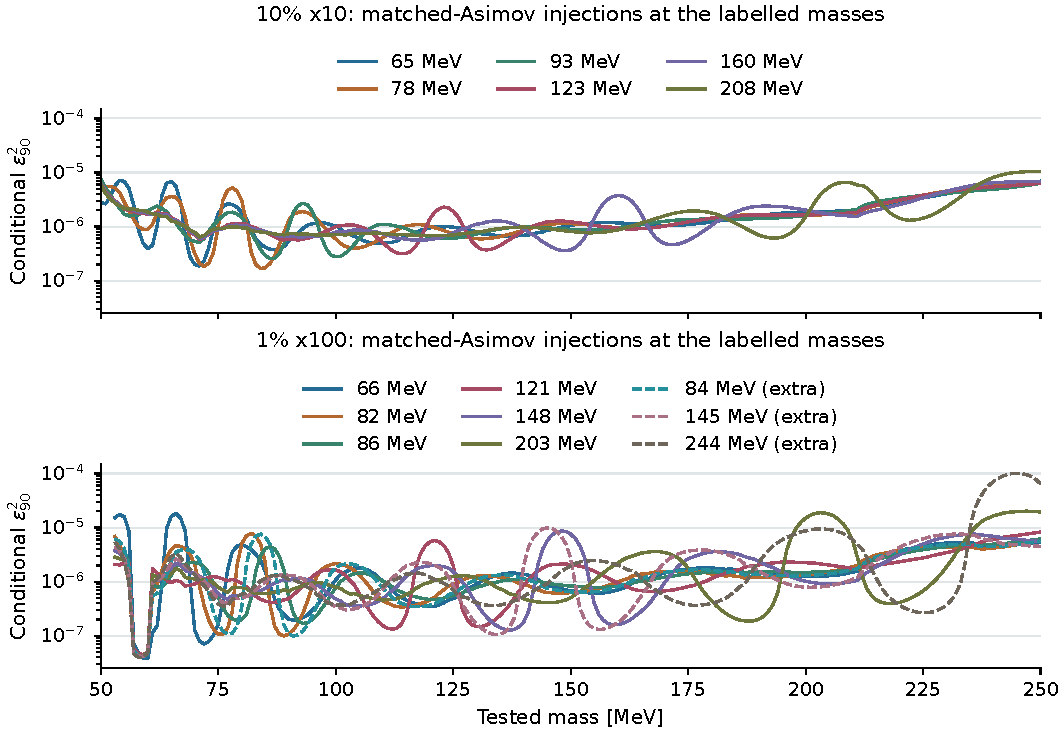
\includegraphics[width=\linewidth]{../figures/fullrange_overview.pdf}\par
\subheading{Count limits and the prompt-density conversion}
The displayed coupling coordinate uses the standard conversion separately for
each tested spectrum $n$:
\begin{equation}
 K_n(m)=\frac{3\pi m f_{\rm rad}^{\rm eff}}{2\alpha}\,\rho_n(m),
 \qquad \epsilon^2_{90,n}(m)=\frac{A_{90,n}(m)}{K_n(m)}\,B_e^{-1}(m).
\end{equation}
Here $f_{\rm rad}^{\rm eff}=0.0477$, $\alpha=1/137$, and $\rho_n$ is the count
density from fractional bin overlap within $\pm1.64\sigma_m$; masses and
density use GeV consistently. Above $2m_\mu=211.316749$ MeV, the inherited
visible branching correction is
$B_e^{-1}=1+\sqrt{1-4u}(1+2u)$, $u=(m_\mu/m)^2$; below threshold it is one.
This explains a physical change in the conversion near 211 MeV.

The echo ledger instead uses $A_{90}/A_{90}^{(b)}$. This is exactly the ratio
of coupling limits evaluated with the same frozen background density in both
numerator and denominator, isolating the fit response from the small change
in the density normalization. Both conversion variants are saved.

\nextpage\heading{Predicted echo locations and depths}
The table records the two selected minima of each matched-Asimov limit ratio. Depth is relative to the scenario's background-only Asimov count limit at the same mass. The listed interval contains saved 1 MeV hypotheses with $R\leq0.90$ connected to that minimum.
\begin{center}\small\setlength{\tabcolsep}{4pt}
\begin{tabular}{@{}lrrrrrrr@{}}\toprule
Option & $m_0$ & Left $m_e$ & Depth & $R\leq0.90$ & Right $m_e$ & Depth & $R\leq0.90$\\
 & [MeV] & [MeV] & [\%] & [MeV] & [MeV] & [\%] & [MeV]\\\midrule
$1\%\times100$ & 66 & 61$^\dagger$ & 92.9 & 57--61 & 72 & 92.2 & 71--76\\
$10\%\times10$ & 65 & 60$^\dagger$ & 79.2 & 58--60 & 70$^\dagger$ & 74.0 & 70--73\\
\addlinespace[2pt]
$1\%\times100$ & 82 & 75 & 84.9 & 71--77 & 89 & 86.7 & 87--94\\
$10\%\times10$ & 78 & 72 & 77.7 & 69--73 & 84 & 78.2 & 83--88\\
\addlinespace[2pt]
$1\%\times100$ & 86 & 79 & 76.7 & 75--81 & 93 & 76.0 & 91--99\\
$10\%\times10$ & 93 & 86 & 62.5 & 83--88 & 100 & 65.2 & 98--105\\
\addlinespace[2pt]
$1\%\times100$ & 121 & 112 & 81.1 & 105--115 & 131 & 80.5 & 127--139\\
$10\%\times10$ & 123 & 115 & 53.3 & 109--117 & 132 & 54.3 & 129--138\\
\addlinespace[2pt]
$1\%\times100$ & 148 & 137 & 83.7 & 129--140 & 160 & 84.2 & 156--170\\
$10\%\times10$ & 160 & 149 & 60.4 & 142--152 & 172 & 61.1 & 168--180\\
\addlinespace[2pt]
$1\%\times100$ & 203 & 189 & 86.8 & 177--192 & 219 & 86.6 & 214--232\\
$10\%\times10$ & 208 & 194 & 60.8 & 185--197 & 224 & 61.2 & 219--234\\
\addlinespace[2pt]
$1\%\times100$ & 84 & 78 & 85.9 & 73--79 & 91 & 86.1 & 89--96\\
$1\%\times100$ & 145 & 135 & 85.7 & 126--138 & 156 & 86.9 & 152--166\\
$1\%\times100$ & 244 & 227 & 92.2 & 214--230 & -- & -- & --\\
\bottomrule\end{tabular}\end{center}
\smallnote{$\dagger$: selected point is a search-flank or scan endpoint. $^*$: no local minimum; the fallback flank minimum is reported. A dash means an unavailable flank or no connected $R\leq0.90$ interval. The 244 MeV injection's right search flank lies outside the scan. A positive depth identifies a depression; a nonpositive depth does not. The additional 1\% injections at 84, 145 and 244 MeV follow the six requested pairs.}
\subheading{The saved spectra and source interpretation}
Every scenario contains a background-only continuum, a target-matched injection, a simple yield-scaled injection and the same 20 toys used in v5.6.0. Only the target-matched injection has toys. The simple yield-scaled amplitude is $a_{\rm yield}=k\max(\widehat a_f,0)$; the matched amplitude was chosen so that its fixed-mass Asimov score equals $\sqrt{k}Z_f$. Agreement with that target is an injection construction, not evidence that the GP satisfies ideal exposure scaling.
The historical 1\% input is the last-used study source, with its own reviewed kernel coordinates and 40--300 MeV conditioning support. The native 10\% option uses its own reviewed states and 36--300 MeV support. The respective limit grids are 53--250 and 50--250 MeV in 1 MeV steps. The 1\% lower-edge control region at 50--52 MeV remains excluded. Both use the inherited fully scaled resolution, 0.625 MeV bins and a $\pm2.25\sigma_m$ fit exclusion.
The exact selection, trigger-category membership, overlap and effective exposure equivalence of the two source samples remain unverified. The source significances inherited from v5.6 are fresh evaluations at archived kernels, rather than verbatim older released values. Numerical-method differences must not be read as exposure effects.
The 1\% injections at 86 and 148 MeV are inherited source-region boundary controls, not interior observed peaks. In particular, the 1\% 86 MeV control is distinct from the native 10\% injection at 93 MeV.
\subheading{What the toy summaries mean}
On each flank, the toy minimum is searched over the same declared interval. The following pages report empirical medians and 16--84\% ranges for its mass. To test persistence at a common location, the ratio summary and threshold count use each toy's ratio at the fixed matched-Asimov echo mass, not at its moving minimum. The plots contain every saved toy curve. These are descriptive summaries of 20 conditional realizations. They are not a background expected band, a simultaneous uncertainty band, or a calibrated confidence interval for the echo.
\nextpage\heading{65 MeV region: $1\%\times100$}
$m_0=66$ MeV, $\sigma_m=2.132$ MeV; $Z_{\rm target}=26.12$, $a_{\rm match}/a_{\rm yield}=1.115$. The deterministic curves and all 20 saved toy limits use fresh GP conditioning.
\par\noindent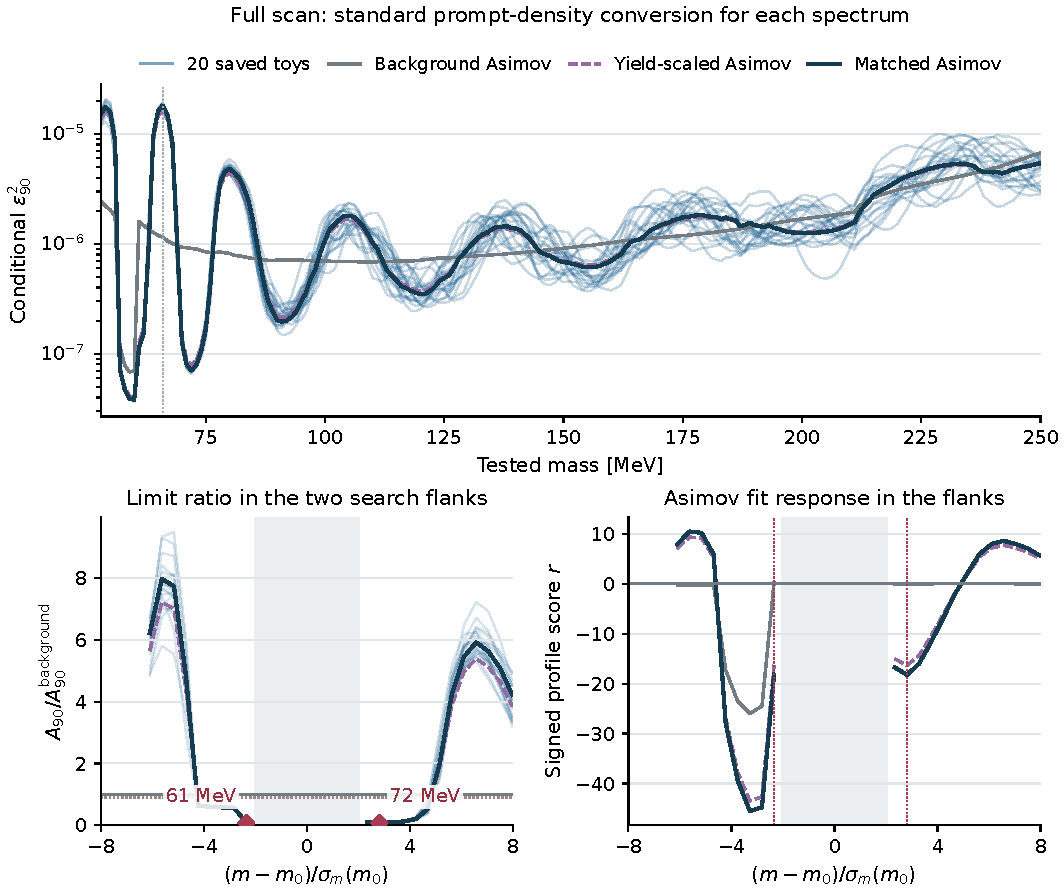
\includegraphics[width=\linewidth]{../figures/one_65.pdf}\par
\smallnote{Top: full-range coupling limits with each spectrum's own prompt density. Lower left: count-limit ratios; diamonds mark the selected matched-Asimov minima and the dotted line is $R=0.90$. Lower right: signed Asimov profile scores with the same line styles. Gray central bands omit $|m-m_0|<2\sigma_m$ from the two flank displays.}
\begin{center}\small\setlength{\tabcolsep}{3pt}
\begin{tabular}{@{}lrrrllr@{}}\toprule
Flank & $m_e$ & Depth & $R\leq0.90$ & Toy mass [MeV] & Toy $R(m_e)$ & $R\leq0.9$\\
 & [MeV] & [\%] & [MeV] & median [16,84\%] & median [16,84\%] & count\\\midrule
Left & 61$^\dagger$ & 92.9 & 57--61 & 61.0 [61.0, 61.0] & 0.07 [0.07, 0.08] & 20/20\\
Right & 72 & 92.2 & 71--76 & 72.0 [72.0, 72.0] & 0.08 [0.08, 0.08] & 20/20\\
\bottomrule\end{tabular}\end{center}
Search bounds after clipping to the scan are left: 53.00--61.74 MeV; right: 70.26--83.05 MeV. $\dagger$ marks an endpoint and $^*$ a fallback minimum; the 1 MeV grid limits position precision.
\nextpage\heading{65 MeV region: $10\%\times10$}
$m_0=65$ MeV, $\sigma_m=2.122$ MeV; $Z_{\rm target}=7.58$, $a_{\rm match}/a_{\rm yield}=1.120$. The deterministic curves and all 20 saved toy limits use fresh GP conditioning.
\par\noindent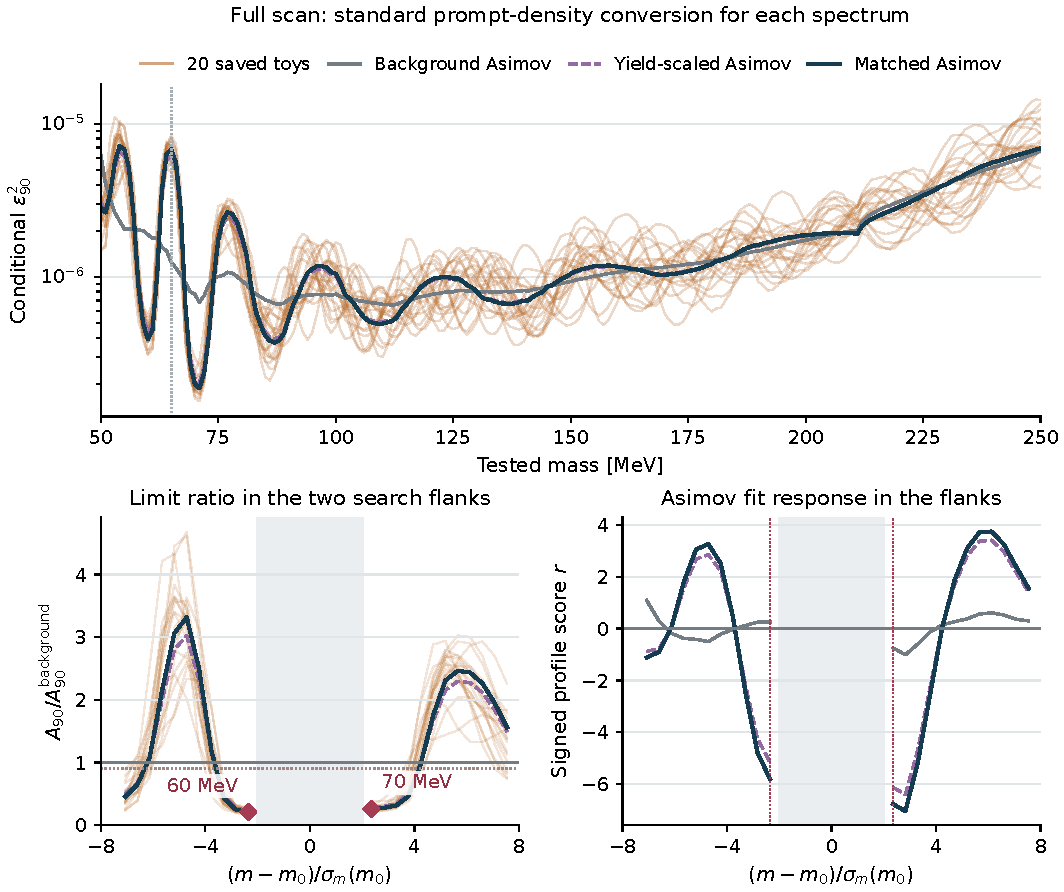
\includegraphics[width=\linewidth]{../figures/ten_65.pdf}\par
\smallnote{Top: full-range coupling limits with each spectrum's own prompt density. Lower left: count-limit ratios; diamonds mark the selected matched-Asimov minima and the dotted line is $R=0.90$. Lower right: signed Asimov profile scores with the same line styles. Gray central bands omit $|m-m_0|<2\sigma_m$ from the two flank displays.}
\begin{center}\small\setlength{\tabcolsep}{3pt}
\begin{tabular}{@{}lrrrllr@{}}\toprule
Flank & $m_e$ & Depth & $R\leq0.90$ & Toy mass [MeV] & Toy $R(m_e)$ & $R\leq0.9$\\
 & [MeV] & [\%] & [MeV] & median [16,84\%] & median [16,84\%] & count\\\midrule
Left & 60$^\dagger$ & 79.2 & 58--60 & 60.0 [60.0, 60.0] & 0.22 [0.20, 0.26] & 20/20\\
Right & 70$^\dagger$ & 74.0 & 70--73 & 70.0 [70.0, 70.0] & 0.25 [0.23, 0.29] & 20/20\\
\bottomrule\end{tabular}\end{center}
Search bounds after clipping to the scan are left: 50.00--60.76 MeV; right: 69.24--81.97 MeV. $\dagger$ marks an endpoint and $^*$ a fallback minimum; the 1 MeV grid limits position precision.
\nextpage\heading{75 MeV region: $1\%\times100$}
$m_0=82$ MeV, $\sigma_m=2.313$ MeV; $Z_{\rm target}=15.32$, $a_{\rm match}/a_{\rm yield}=1.095$. The deterministic curves and all 20 saved toy limits use fresh GP conditioning.
\par\noindent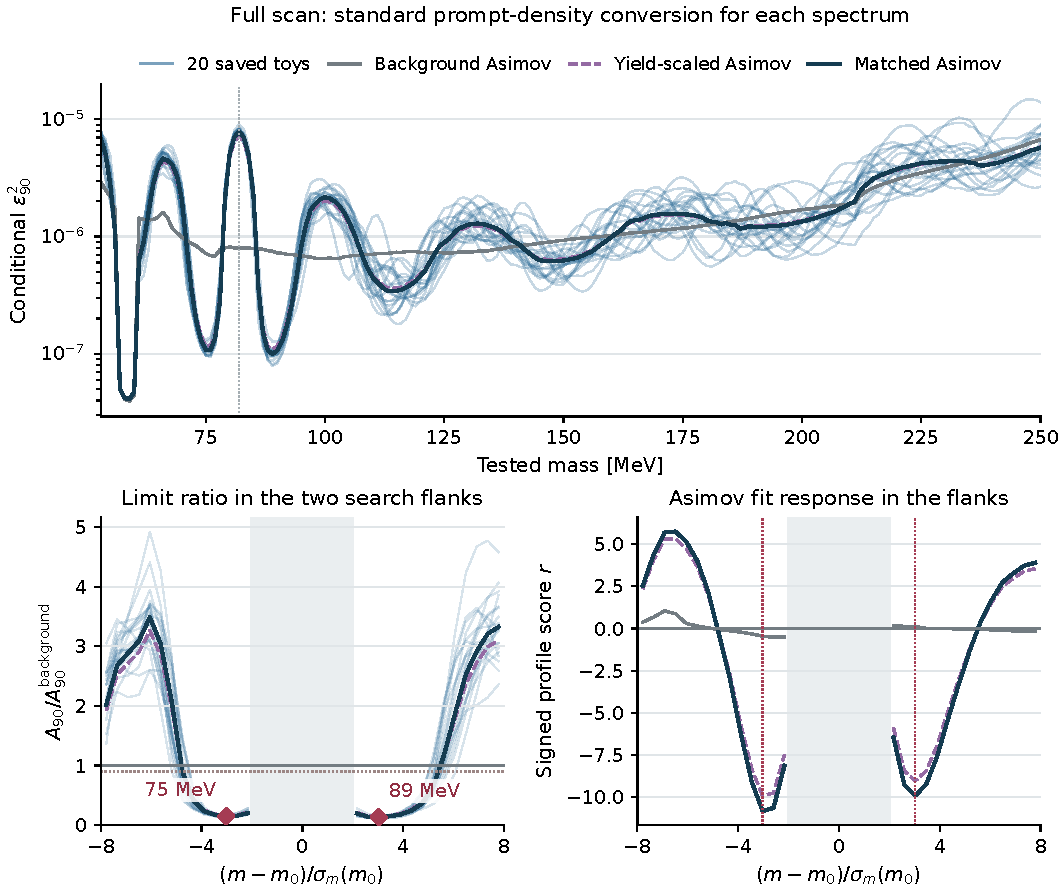
\includegraphics[width=\linewidth]{../figures/one_75.pdf}\par
\smallnote{Top: full-range coupling limits with each spectrum's own prompt density. Lower left: count-limit ratios; diamonds mark the selected matched-Asimov minima and the dotted line is $R=0.90$. Lower right: signed Asimov profile scores with the same line styles. Gray central bands omit $|m-m_0|<2\sigma_m$ from the two flank displays.}
\begin{center}\small\setlength{\tabcolsep}{3pt}
\begin{tabular}{@{}lrrrllr@{}}\toprule
Flank & $m_e$ & Depth & $R\leq0.90$ & Toy mass [MeV] & Toy $R(m_e)$ & $R\leq0.9$\\
 & [MeV] & [\%] & [MeV] & median [16,84\%] & median [16,84\%] & count\\\midrule
Left & 75 & 84.9 & 71--77 & 75.0 [75.0, 75.0] & 0.15 [0.14, 0.16] & 20/20\\
Right & 89 & 86.7 & 87--94 & 89.0 [89.0, 89.0] & 0.13 [0.13, 0.14] & 20/20\\
\bottomrule\end{tabular}\end{center}
Search bounds after clipping to the scan are left: 63.50--77.37 MeV; right: 86.63--100.50 MeV. $\dagger$ marks an endpoint and $^*$ a fallback minimum; the 1 MeV grid limits position precision.
\nextpage\heading{75 MeV region: $10\%\times10$}
$m_0=78$ MeV, $\sigma_m=2.263$ MeV; $Z_{\rm target}=8.88$, $a_{\rm match}/a_{\rm yield}=1.059$. The deterministic curves and all 20 saved toy limits use fresh GP conditioning.
\par\noindent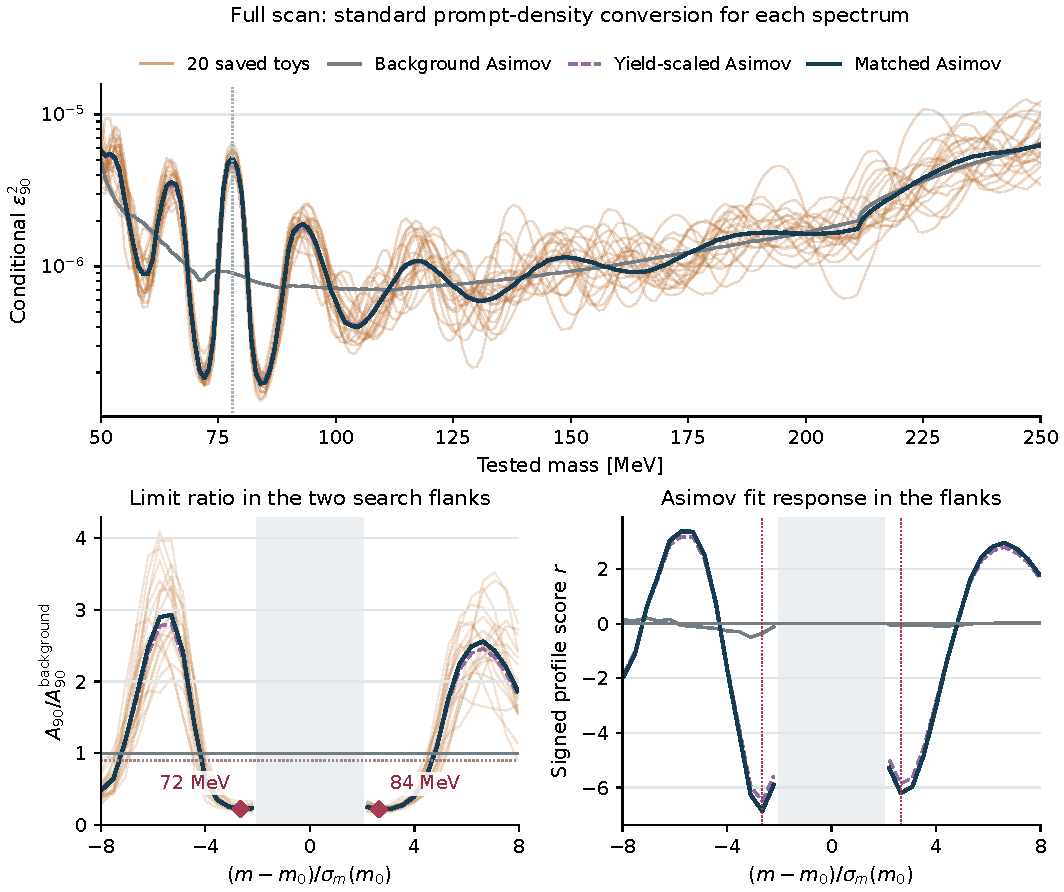
\includegraphics[width=\linewidth]{../figures/ten_75.pdf}\par
\smallnote{Top: full-range coupling limits with each spectrum's own prompt density. Lower left: count-limit ratios; diamonds mark the selected matched-Asimov minima and the dotted line is $R=0.90$. Lower right: signed Asimov profile scores with the same line styles. Gray central bands omit $|m-m_0|<2\sigma_m$ from the two flank displays.}
\begin{center}\small\setlength{\tabcolsep}{3pt}
\begin{tabular}{@{}lrrrllr@{}}\toprule
Flank & $m_e$ & Depth & $R\leq0.90$ & Toy mass [MeV] & Toy $R(m_e)$ & $R\leq0.9$\\
 & [MeV] & [\%] & [MeV] & median [16,84\%] & median [16,84\%] & count\\\midrule
Left & 72 & 77.7 & 69--73 & 72.0 [72.0, 73.0] & 0.22 [0.20, 0.26] & 20/20\\
Right & 84 & 78.2 & 83--88 & 84.0 [84.0, 85.0] & 0.22 [0.19, 0.25] & 20/20\\
\bottomrule\end{tabular}\end{center}
Search bounds after clipping to the scan are left: 59.89--73.47 MeV; right: 82.53--96.11 MeV. $\dagger$ marks an endpoint and $^*$ a fallback minimum; the 1 MeV grid limits position precision.
\nextpage\heading{92 MeV region: $1\%\times100$}
$m_0=86$ MeV, $\sigma_m=2.365$ MeV; $Z_{\rm target}=8.61$, $a_{\rm match}/a_{\rm yield}=1.078$. The deterministic curves and all 20 saved toy limits use fresh GP conditioning. Inherited source-region boundary control.
\par\noindent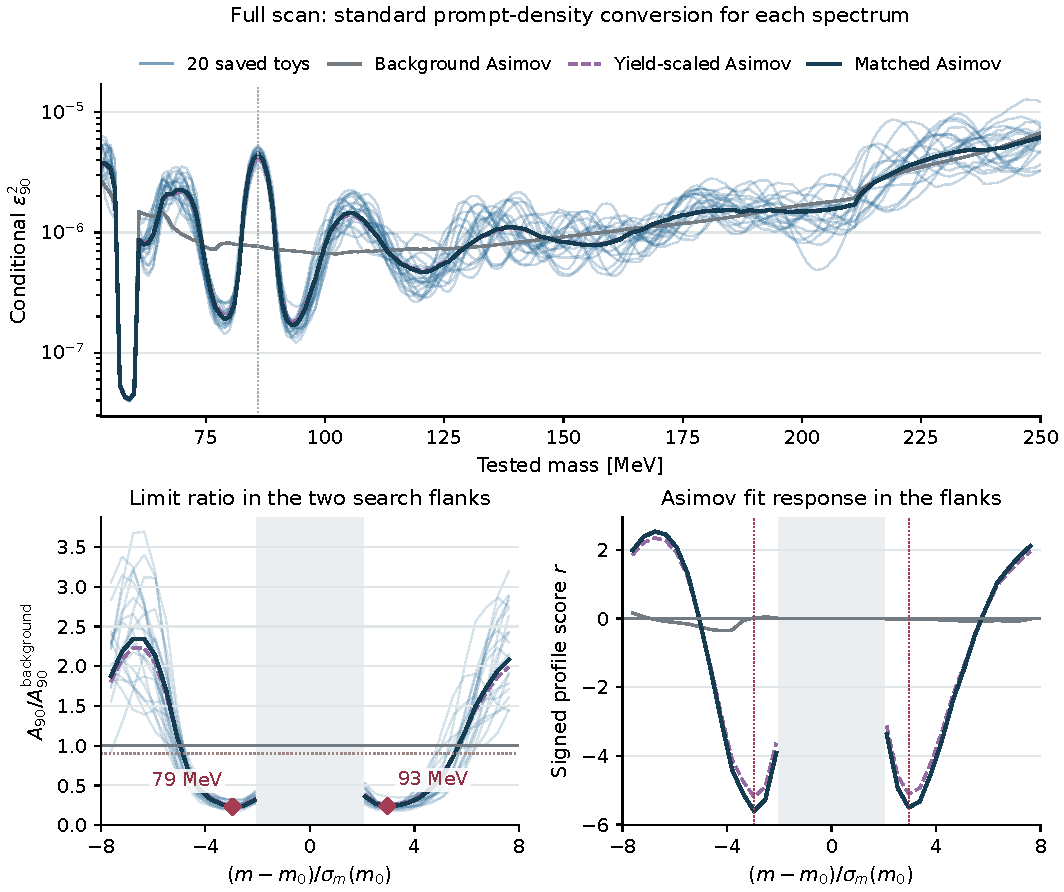
\includegraphics[width=\linewidth]{../figures/one_92.pdf}\par
\smallnote{Top: full-range coupling limits with each spectrum's own prompt density. Lower left: count-limit ratios; diamonds mark the selected matched-Asimov minima and the dotted line is $R=0.90$. Lower right: signed Asimov profile scores with the same line styles. Gray central bands omit $|m-m_0|<2\sigma_m$ from the two flank displays.}
\begin{center}\small\setlength{\tabcolsep}{3pt}
\begin{tabular}{@{}lrrrllr@{}}\toprule
Flank & $m_e$ & Depth & $R\leq0.90$ & Toy mass [MeV] & Toy $R(m_e)$ & $R\leq0.9$\\
 & [MeV] & [\%] & [MeV] & median [16,84\%] & median [16,84\%] & count\\\midrule
Left & 79 & 76.7 & 75--81 & 79.0 [79.0, 79.0] & 0.24 [0.21, 0.29] & 20/20\\
Right & 93 & 76.0 & 91--99 & 93.5 [93.0, 94.0] & 0.24 [0.20, 0.26] & 20/20\\
\bottomrule\end{tabular}\end{center}
Search bounds after clipping to the scan are left: 67.08--81.27 MeV; right: 90.73--104.92 MeV. $\dagger$ marks an endpoint and $^*$ a fallback minimum; the 1 MeV grid limits position precision.
\nextpage\heading{92 MeV region: $10\%\times10$}
$m_0=93$ MeV, $\sigma_m=2.463$ MeV; $Z_{\rm target}=4.77$, $a_{\rm match}/a_{\rm yield}=1.071$. The deterministic curves and all 20 saved toy limits use fresh GP conditioning.
\par\noindent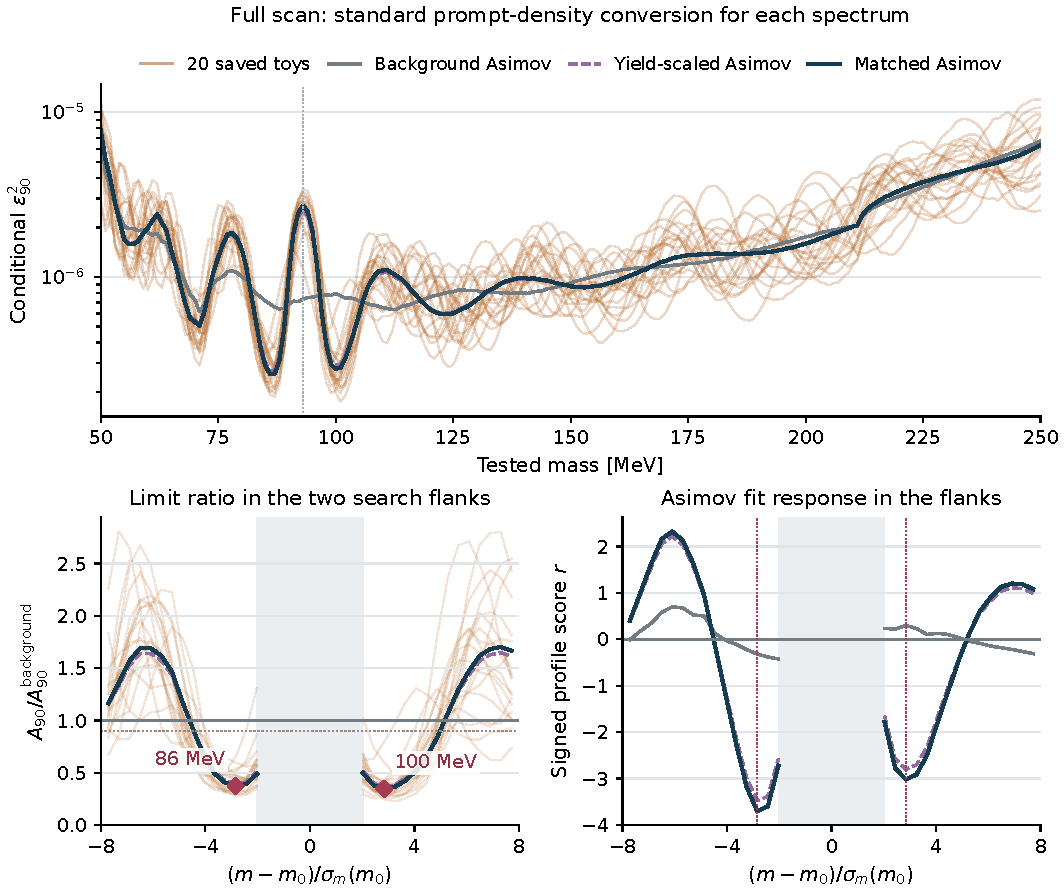
\includegraphics[width=\linewidth]{../figures/ten_92.pdf}\par
\smallnote{Top: full-range coupling limits with each spectrum's own prompt density. Lower left: count-limit ratios; diamonds mark the selected matched-Asimov minima and the dotted line is $R=0.90$. Lower right: signed Asimov profile scores with the same line styles. Gray central bands omit $|m-m_0|<2\sigma_m$ from the two flank displays.}
\begin{center}\small\setlength{\tabcolsep}{3pt}
\begin{tabular}{@{}lrrrllr@{}}\toprule
Flank & $m_e$ & Depth & $R\leq0.90$ & Toy mass [MeV] & Toy $R(m_e)$ & $R\leq0.9$\\
 & [MeV] & [\%] & [MeV] & median [16,84\%] & median [16,84\%] & count\\\midrule
Left & 86 & 62.5 & 83--88 & 86.0 [85.0, 87.0] & 0.41 [0.31, 0.51] & 20/20\\
Right & 100 & 65.2 & 98--105 & 100.0 [99.0, 101.0] & 0.33 [0.29, 0.43] & 20/20\\
\bottomrule\end{tabular}\end{center}
Search bounds after clipping to the scan are left: 73.30--88.07 MeV; right: 97.93--112.70 MeV. $\dagger$ marks an endpoint and $^*$ a fallback minimum; the 1 MeV grid limits position precision.
\nextpage\heading{120 MeV region: $1\%\times100$}
$m_0=121$ MeV, $\sigma_m=2.939$ MeV; $Z_{\rm target}=11.94$, $a_{\rm match}/a_{\rm yield}=1.073$. The deterministic curves and all 20 saved toy limits use fresh GP conditioning.
\par\noindent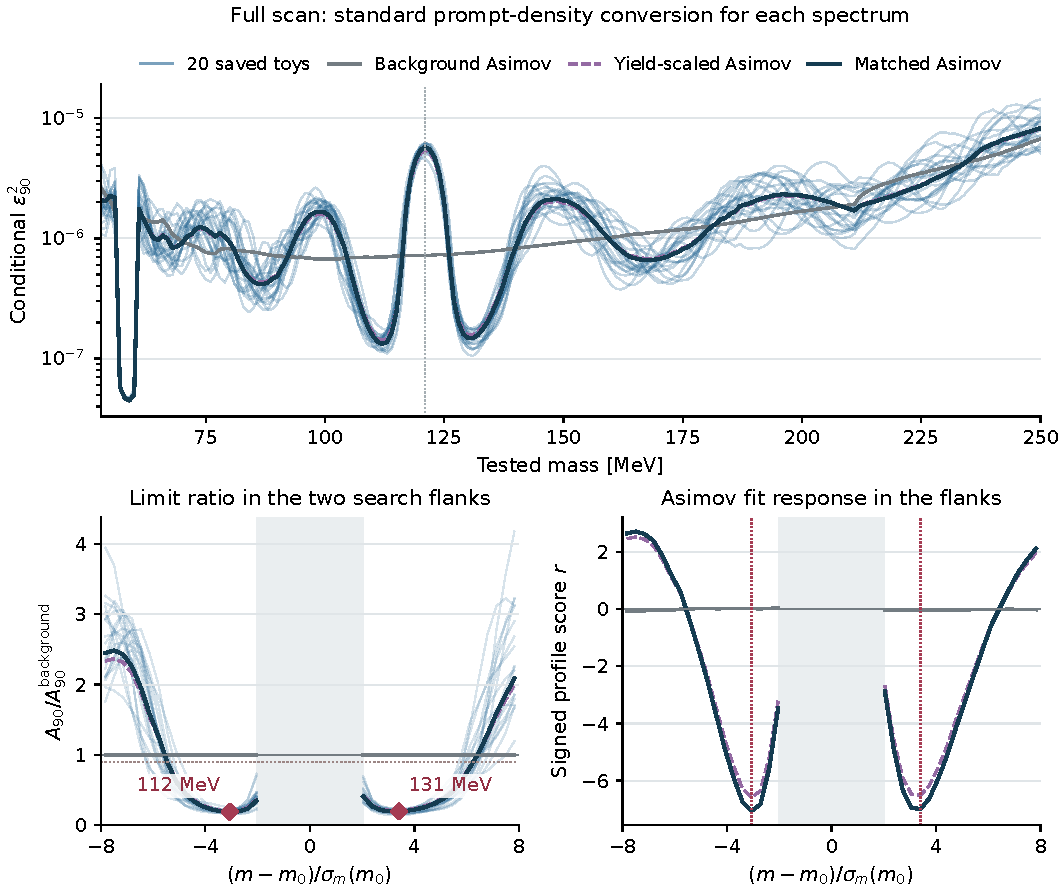
\includegraphics[width=\linewidth]{../figures/one_120.pdf}\par
\smallnote{Top: full-range coupling limits with each spectrum's own prompt density. Lower left: count-limit ratios; diamonds mark the selected matched-Asimov minima and the dotted line is $R=0.90$. Lower right: signed Asimov profile scores with the same line styles. Gray central bands omit $|m-m_0|<2\sigma_m$ from the two flank displays.}
\begin{center}\small\setlength{\tabcolsep}{3pt}
\begin{tabular}{@{}lrrrllr@{}}\toprule
Flank & $m_e$ & Depth & $R\leq0.90$ & Toy mass [MeV] & Toy $R(m_e)$ & $R\leq0.9$\\
 & [MeV] & [\%] & [MeV] & median [16,84\%] & median [16,84\%] & count\\\midrule
Left & 112 & 81.1 & 105--115 & 112.0 [111.0, 112.0] & 0.20 [0.17, 0.22] & 20/20\\
Right & 131 & 80.5 & 127--139 & 131.0 [130.0, 132.0] & 0.20 [0.16, 0.23] & 20/20\\
\bottomrule\end{tabular}\end{center}
Search bounds after clipping to the scan are left: 97.49--115.12 MeV; right: 126.88--144.51 MeV. $\dagger$ marks an endpoint and $^*$ a fallback minimum; the 1 MeV grid limits position precision.
\nextpage\heading{120 MeV region: $10\%\times10$}
$m_0=123$ MeV, $\sigma_m=2.978$ MeV; $Z_{\rm target}=3.74$, $a_{\rm match}/a_{\rm yield}=1.028$. The deterministic curves and all 20 saved toy limits use fresh GP conditioning.
\par\noindent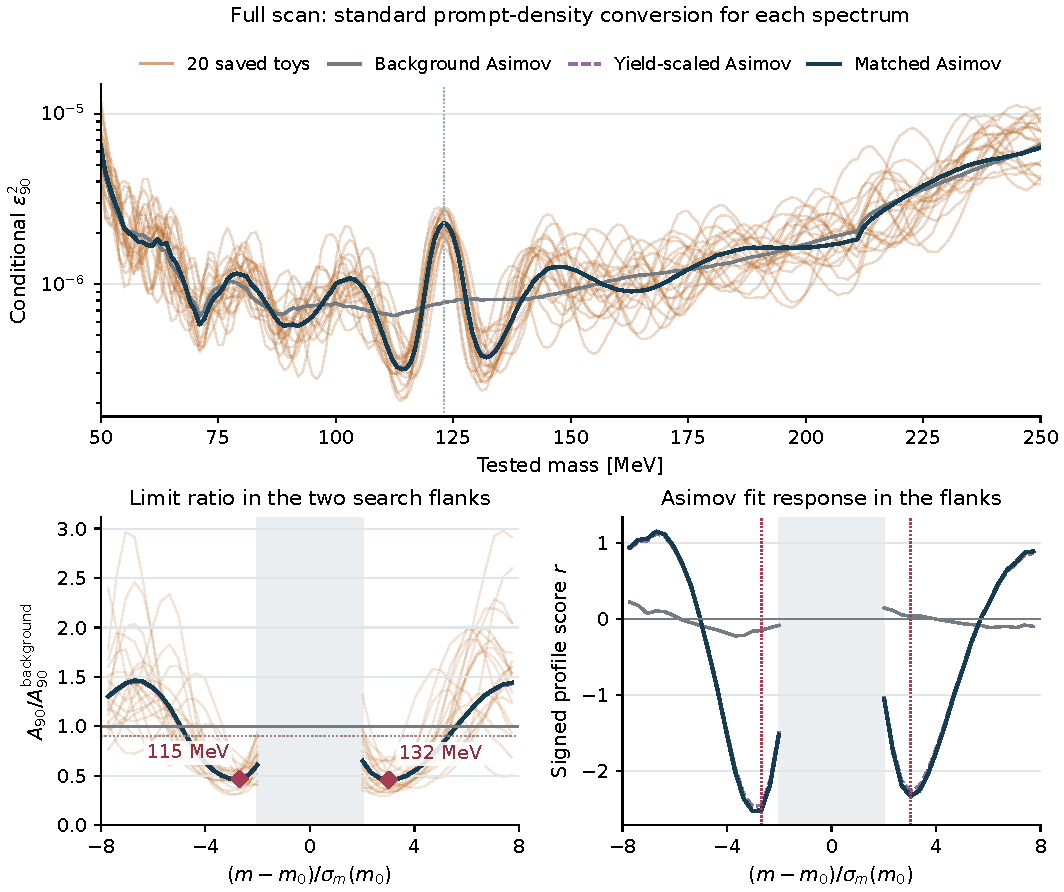
\includegraphics[width=\linewidth]{../figures/ten_120.pdf}\par
\smallnote{Top: full-range coupling limits with each spectrum's own prompt density. Lower left: count-limit ratios; diamonds mark the selected matched-Asimov minima and the dotted line is $R=0.90$. Lower right: signed Asimov profile scores with the same line styles. Gray central bands omit $|m-m_0|<2\sigma_m$ from the two flank displays.}
\begin{center}\small\setlength{\tabcolsep}{3pt}
\begin{tabular}{@{}lrrrllr@{}}\toprule
Flank & $m_e$ & Depth & $R\leq0.90$ & Toy mass [MeV] & Toy $R(m_e)$ & $R\leq0.9$\\
 & [MeV] & [\%] & [MeV] & median [16,84\%] & median [16,84\%] & count\\\midrule
Left & 115 & 53.3 & 109--117 & 114.5 [112.1, 115.0] & 0.51 [0.37, 0.56] & 20/20\\
Right & 132 & 54.3 & 129--138 & 132.0 [131.0, 133.0] & 0.45 [0.35, 0.62] & 20/20\\
\bottomrule\end{tabular}\end{center}
Search bounds after clipping to the scan are left: 99.17--117.04 MeV; right: 128.96--146.83 MeV. $\dagger$ marks an endpoint and $^*$ a fallback minimum; the 1 MeV grid limits position precision.
\nextpage\heading{160 MeV region: $1\%\times100$}
$m_0=148$ MeV, $\sigma_m=3.526$ MeV; $Z_{\rm target}=14.66$, $a_{\rm match}/a_{\rm yield}=1.079$. The deterministic curves and all 20 saved toy limits use fresh GP conditioning. Inherited source-region boundary control.
\par\noindent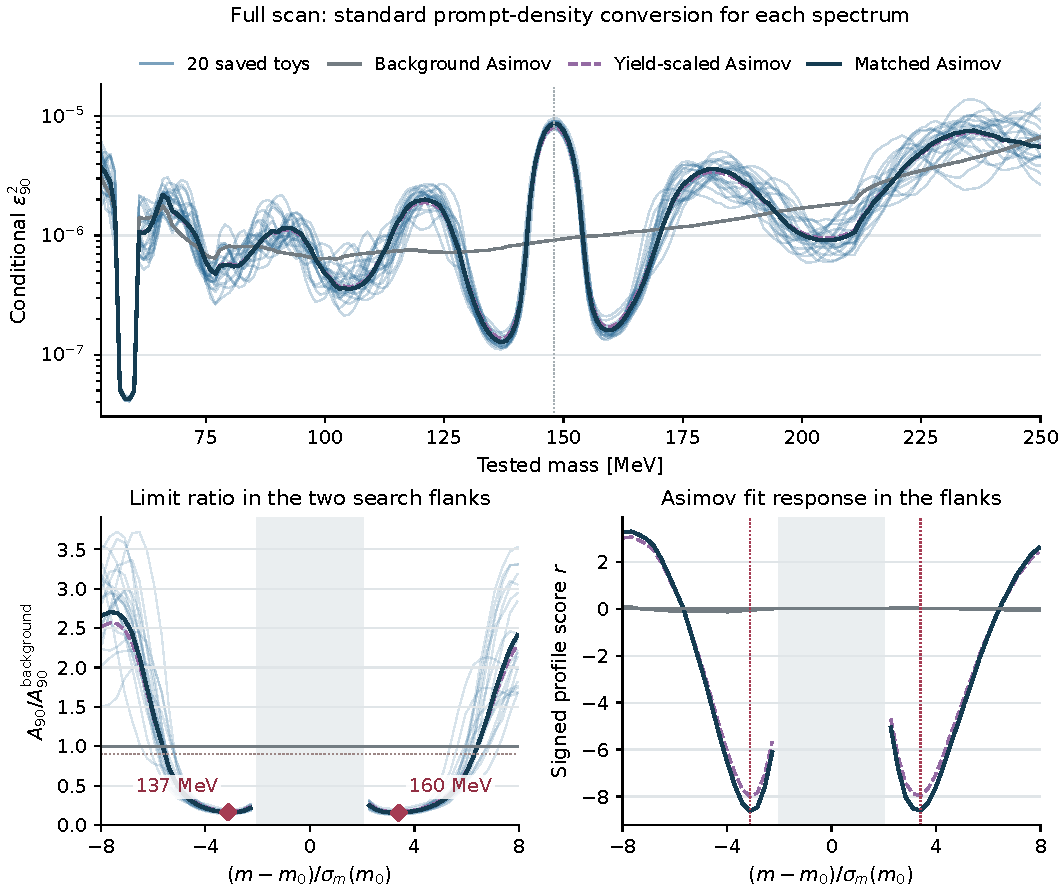
\includegraphics[width=\linewidth]{../figures/one_160.pdf}\par
\smallnote{Top: full-range coupling limits with each spectrum's own prompt density. Lower left: count-limit ratios; diamonds mark the selected matched-Asimov minima and the dotted line is $R=0.90$. Lower right: signed Asimov profile scores with the same line styles. Gray central bands omit $|m-m_0|<2\sigma_m$ from the two flank displays.}
\begin{center}\small\setlength{\tabcolsep}{3pt}
\begin{tabular}{@{}lrrrllr@{}}\toprule
Flank & $m_e$ & Depth & $R\leq0.90$ & Toy mass [MeV] & Toy $R(m_e)$ & $R\leq0.9$\\
 & [MeV] & [\%] & [MeV] & median [16,84\%] & median [16,84\%] & count\\\midrule
Left & 137 & 83.7 & 129--140 & 137.5 [137.0, 138.0] & 0.16 [0.15, 0.18] & 20/20\\
Right & 160 & 84.2 & 156--170 & 159.5 [159.0, 160.0] & 0.15 [0.14, 0.16] & 20/20\\
\bottomrule\end{tabular}\end{center}
Search bounds after clipping to the scan are left: 119.79--140.95 MeV; right: 155.05--176.21 MeV. $\dagger$ marks an endpoint and $^*$ a fallback minimum; the 1 MeV grid limits position precision.
\nextpage\heading{160 MeV region: $10\%\times10$}
$m_0=160$ MeV, $\sigma_m=3.827$ MeV; $Z_{\rm target}=4.71$, $a_{\rm match}/a_{\rm yield}=1.039$. The deterministic curves and all 20 saved toy limits use fresh GP conditioning.
\par\noindent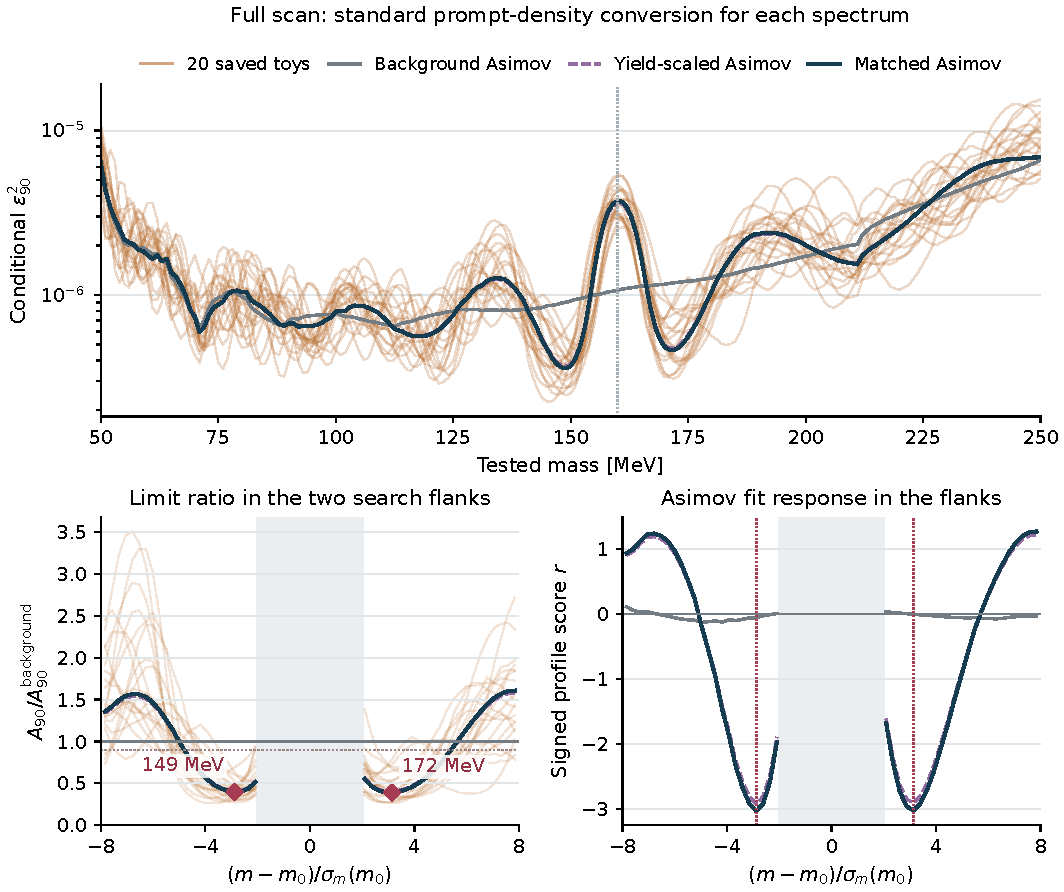
\includegraphics[width=\linewidth]{../figures/ten_160.pdf}\par
\smallnote{Top: full-range coupling limits with each spectrum's own prompt density. Lower left: count-limit ratios; diamonds mark the selected matched-Asimov minima and the dotted line is $R=0.90$. Lower right: signed Asimov profile scores with the same line styles. Gray central bands omit $|m-m_0|<2\sigma_m$ from the two flank displays.}
\begin{center}\small\setlength{\tabcolsep}{3pt}
\begin{tabular}{@{}lrrrllr@{}}\toprule
Flank & $m_e$ & Depth & $R\leq0.90$ & Toy mass [MeV] & Toy $R(m_e)$ & $R\leq0.9$\\
 & [MeV] & [\%] & [MeV] & median [16,84\%] & median [16,84\%] & count\\\midrule
Left & 149 & 60.4 & 142--152 & 149.0 [146.0, 151.0] & 0.43 [0.31, 0.52] & 20/20\\
Right & 172 & 61.1 & 168--180 & 172.0 [170.0, 173.0] & 0.41 [0.33, 0.67] & 20/20\\
\bottomrule\end{tabular}\end{center}
Search bounds after clipping to the scan are left: 129.39--152.35 MeV; right: 167.65--190.61 MeV. $\dagger$ marks an endpoint and $^*$ a fallback minimum; the 1 MeV grid limits position precision.
\nextpage\heading{210 MeV region: $1\%\times100$}
$m_0=203$ MeV, $\sigma_m=5.108$ MeV; $Z_{\rm target}=16.87$, $a_{\rm match}/a_{\rm yield}=1.089$. The deterministic curves and all 20 saved toy limits use fresh GP conditioning.
\par\noindent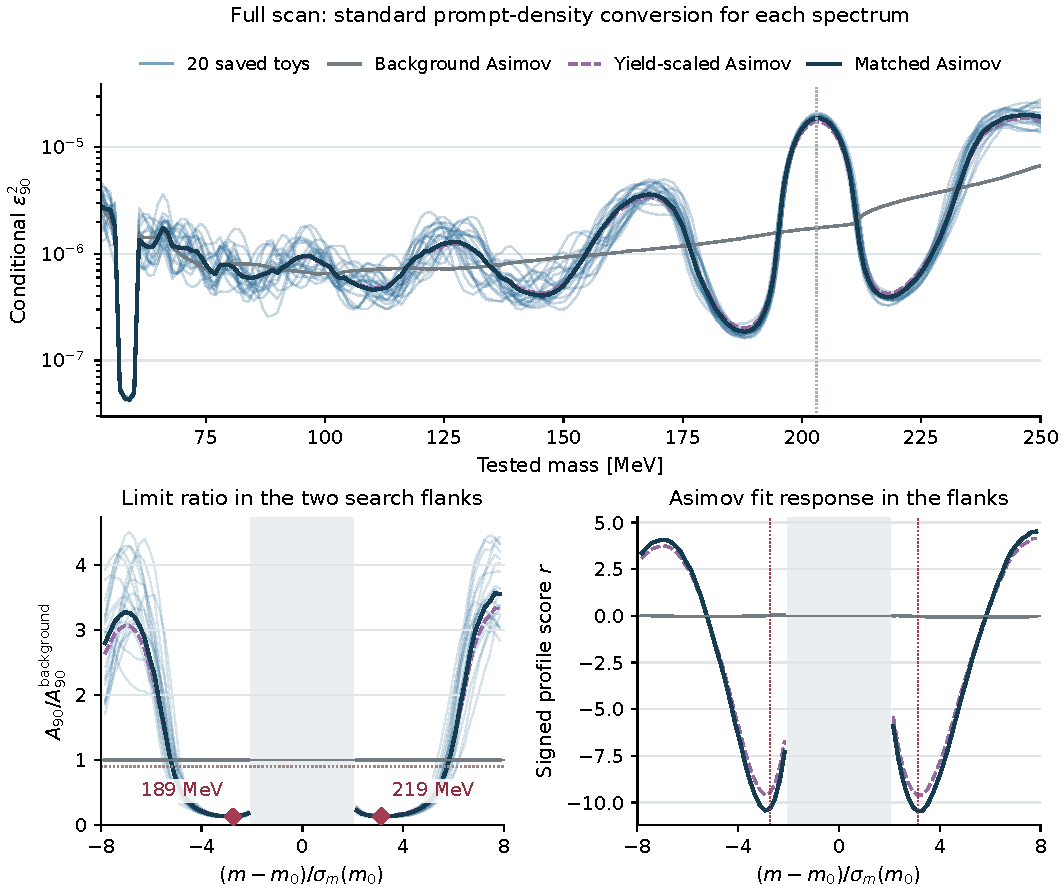
\includegraphics[width=\linewidth]{../figures/one_210.pdf}\par
\smallnote{Top: full-range coupling limits with each spectrum's own prompt density. Lower left: count-limit ratios; diamonds mark the selected matched-Asimov minima and the dotted line is $R=0.90$. Lower right: signed Asimov profile scores with the same line styles. Gray central bands omit $|m-m_0|<2\sigma_m$ from the two flank displays.}
\begin{center}\small\setlength{\tabcolsep}{3pt}
\begin{tabular}{@{}lrrrllr@{}}\toprule
Flank & $m_e$ & Depth & $R\leq0.90$ & Toy mass [MeV] & Toy $R(m_e)$ & $R\leq0.9$\\
 & [MeV] & [\%] & [MeV] & median [16,84\%] & median [16,84\%] & count\\\midrule
Left & 189 & 86.8 & 177--192 & 188.0 [188.0, 189.0] & 0.13 [0.12, 0.14] & 20/20\\
Right & 219 & 86.6 & 214--232 & 219.0 [219.0, 220.0] & 0.13 [0.12, 0.14] & 20/20\\
\bottomrule\end{tabular}\end{center}
Search bounds after clipping to the scan are left: 162.14--192.78 MeV; right: 213.22--243.86 MeV. $\dagger$ marks an endpoint and $^*$ a fallback minimum; the 1 MeV grid limits position precision.
\nextpage\heading{210 MeV region: $10\%\times10$}
$m_0=208$ MeV, $\sigma_m=5.278$ MeV; $Z_{\rm target}=4.46$, $a_{\rm match}/a_{\rm yield}=1.073$. The deterministic curves and all 20 saved toy limits use fresh GP conditioning.
\par\noindent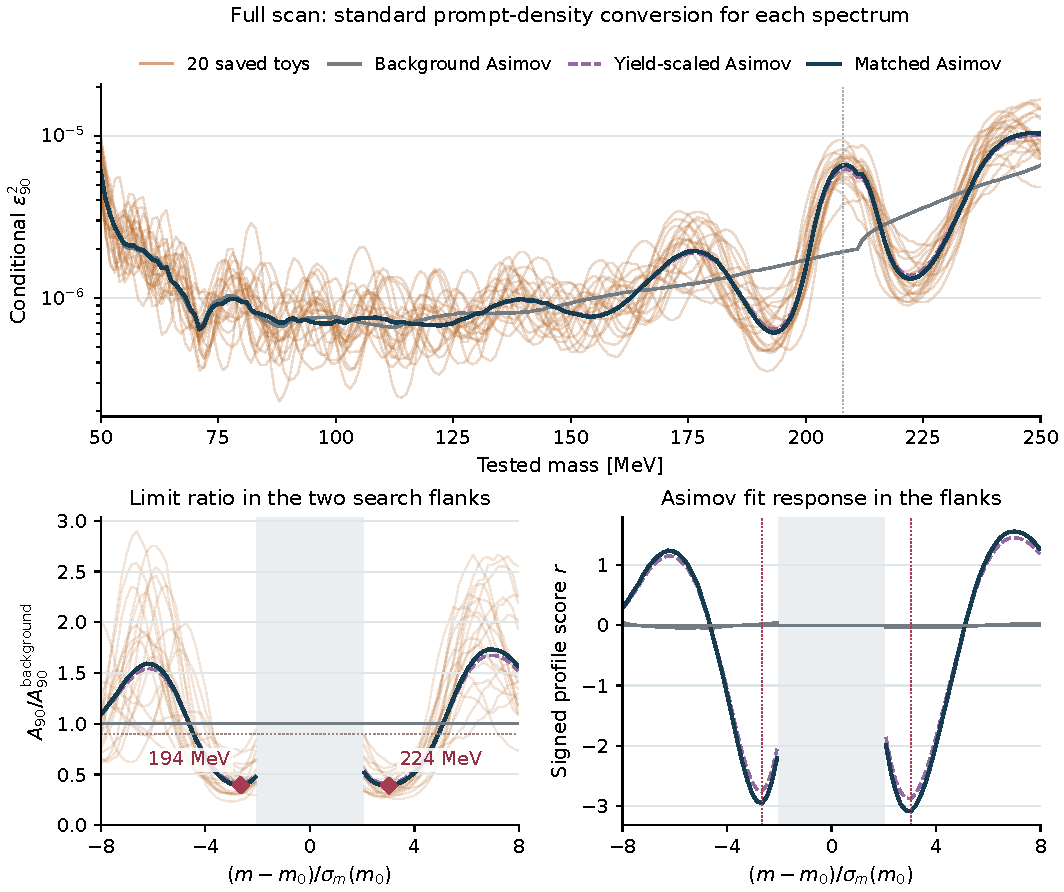
\includegraphics[width=\linewidth]{../figures/ten_210.pdf}\par
\smallnote{Top: full-range coupling limits with each spectrum's own prompt density. Lower left: count-limit ratios; diamonds mark the selected matched-Asimov minima and the dotted line is $R=0.90$. Lower right: signed Asimov profile scores with the same line styles. Gray central bands omit $|m-m_0|<2\sigma_m$ from the two flank displays.}
\begin{center}\small\setlength{\tabcolsep}{3pt}
\begin{tabular}{@{}lrrrllr@{}}\toprule
Flank & $m_e$ & Depth & $R\leq0.90$ & Toy mass [MeV] & Toy $R(m_e)$ & $R\leq0.9$\\
 & [MeV] & [\%] & [MeV] & median [16,84\%] & median [16,84\%] & count\\\midrule
Left & 194 & 60.8 & 185--197 & 193.0 [189.0, 195.0] & 0.41 [0.32, 0.56] & 20/20\\
Right & 224 & 61.2 & 219--234 & 224.0 [222.0, 226.0] & 0.37 [0.30, 0.48] & 20/20\\
\bottomrule\end{tabular}\end{center}
Search bounds after clipping to the scan are left: 165.78--197.44 MeV; right: 218.56--250.00 MeV. $\dagger$ marks an endpoint and $^*$ a fallback minimum; the 1 MeV grid limits position precision.
\nextpage\heading{Additional 1\% injection: 84 MeV}
$m_0=84$ MeV, $\sigma_m=2.339$ MeV; $Z_{\rm target}=15.33$, $a_{\rm match}/a_{\rm yield}=1.092$. The deterministic curves and all 20 saved toy limits use fresh GP conditioning.
\par\noindent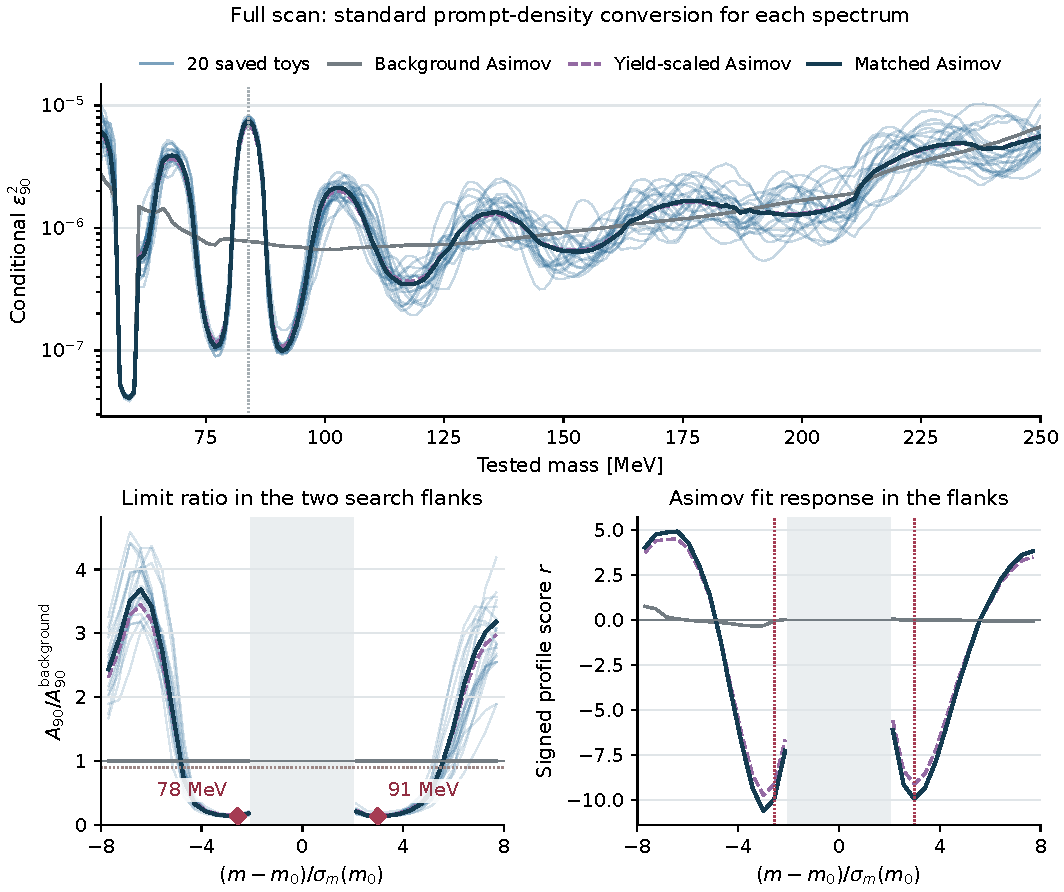
\includegraphics[width=\linewidth]{../figures/one_extra84.pdf}\par
\smallnote{Top: full-range coupling limits with each spectrum's own prompt density. Lower left: count-limit ratios; diamonds mark the selected matched-Asimov minima and the dotted line is $R=0.90$. Lower right: signed Asimov profile scores with the same line styles. Gray central bands omit $|m-m_0|<2\sigma_m$ from the two flank displays.}
\begin{center}\small\setlength{\tabcolsep}{3pt}
\begin{tabular}{@{}lrrrllr@{}}\toprule
Flank & $m_e$ & Depth & $R\leq0.90$ & Toy mass [MeV] & Toy $R(m_e)$ & $R\leq0.9$\\
 & [MeV] & [\%] & [MeV] & median [16,84\%] & median [16,84\%] & count\\\midrule
Left & 78 & 85.9 & 73--79 & 78.0 [78.0, 78.0] & 0.14 [0.13, 0.15] & 20/20\\
Right & 91 & 86.1 & 89--96 & 91.0 [91.0, 91.0] & 0.14 [0.13, 0.15] & 20/20\\
\bottomrule\end{tabular}\end{center}
Search bounds after clipping to the scan are left: 65.29--79.32 MeV; right: 88.68--102.71 MeV. $\dagger$ marks an endpoint and $^*$ a fallback minimum; the 1 MeV grid limits position precision.
\nextpage\heading{Additional 1\% injection: 145 MeV}
$m_0=145$ MeV, $\sigma_m=3.454$ MeV; $Z_{\rm target}=17.32$, $a_{\rm match}/a_{\rm yield}=1.078$. The deterministic curves and all 20 saved toy limits use fresh GP conditioning.
\par\noindent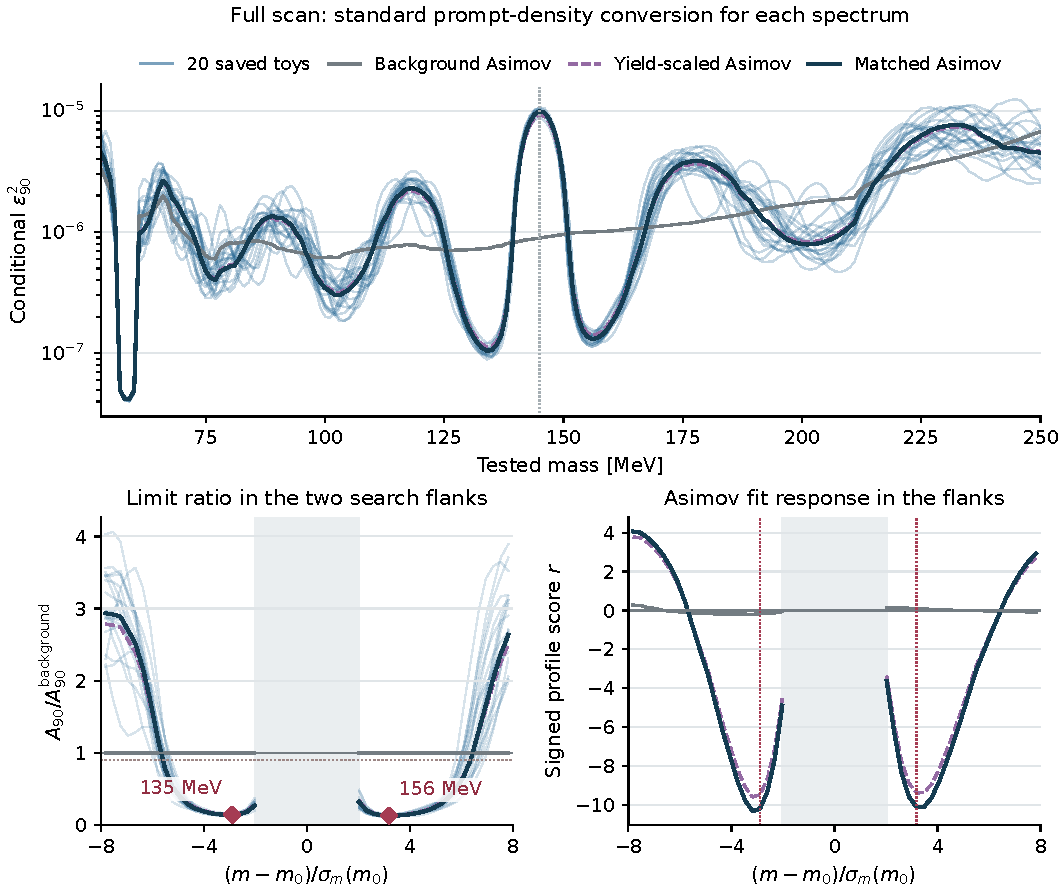
\includegraphics[width=\linewidth]{../figures/one_extra145.pdf}\par
\smallnote{Top: full-range coupling limits with each spectrum's own prompt density. Lower left: count-limit ratios; diamonds mark the selected matched-Asimov minima and the dotted line is $R=0.90$. Lower right: signed Asimov profile scores with the same line styles. Gray central bands omit $|m-m_0|<2\sigma_m$ from the two flank displays.}
\begin{center}\small\setlength{\tabcolsep}{3pt}
\begin{tabular}{@{}lrrrllr@{}}\toprule
Flank & $m_e$ & Depth & $R\leq0.90$ & Toy mass [MeV] & Toy $R(m_e)$ & $R\leq0.9$\\
 & [MeV] & [\%] & [MeV] & median [16,84\%] & median [16,84\%] & count\\\midrule
Left & 135 & 85.7 & 126--138 & 134.0 [134.0, 135.0] & 0.14 [0.13, 0.15] & 20/20\\
Right & 156 & 86.9 & 152--166 & 156.0 [156.0, 157.0] & 0.14 [0.12, 0.14] & 20/20\\
\bottomrule\end{tabular}\end{center}
Search bounds after clipping to the scan are left: 117.36--138.09 MeV; right: 151.91--172.64 MeV. $\dagger$ marks an endpoint and $^*$ a fallback minimum; the 1 MeV grid limits position precision.
\nextpage\heading{Additional 1\% injection: 244 MeV}
$m_0=244$ MeV, $\sigma_m=6.625$ MeV; $Z_{\rm target}=28.61$, $a_{\rm match}/a_{\rm yield}=1.131$. The deterministic curves and all 20 saved toy limits use fresh GP conditioning.
\par\noindent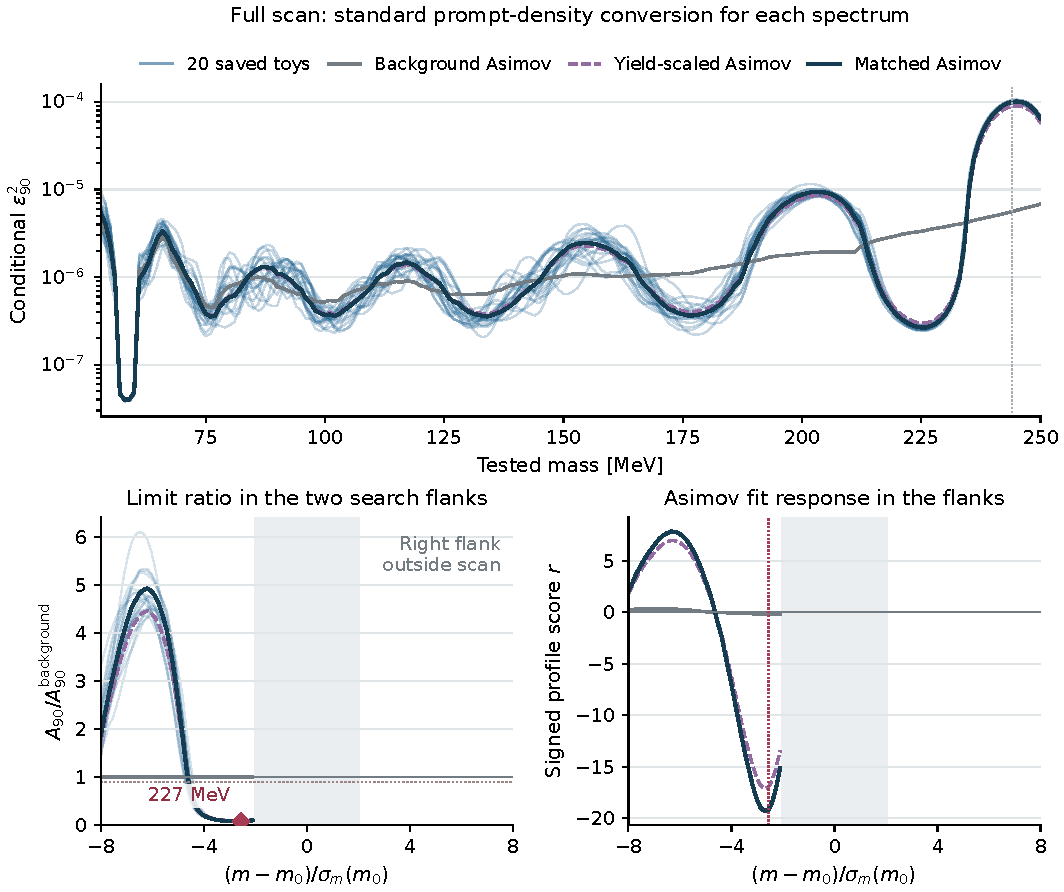
\includegraphics[width=\linewidth]{../figures/one_extra244.pdf}\par
\smallnote{Top: full-range coupling limits with each spectrum's own prompt density. Lower left: count-limit ratios; diamonds mark the selected matched-Asimov minima and the dotted line is $R=0.90$. Lower right: signed Asimov profile scores with the same line styles. Gray central bands omit $|m-m_0|<2\sigma_m$ from the two flank displays.}
\begin{center}\small\setlength{\tabcolsep}{3pt}
\begin{tabular}{@{}lrrrllr@{}}\toprule
Flank & $m_e$ & Depth & $R\leq0.90$ & Toy mass [MeV] & Toy $R(m_e)$ & $R\leq0.9$\\
 & [MeV] & [\%] & [MeV] & median [16,84\%] & median [16,84\%] & count\\\midrule
Left & 227 & 92.2 & 214--230 & 226.0 [226.0, 227.0] & 0.08 [0.07, 0.08] & 20/20\\
Right & \multicolumn{6}{l}{Search flank outside the saved mass scan.}\\
\bottomrule\end{tabular}\end{center}
Search bounds after clipping to the scan are left: 191.00--230.75 MeV. $\dagger$ marks an endpoint and $^*$ a fallback minimum; the 1 MeV grid limits position precision.
\nextpage\heading{Frozen forecast and reproducibility}
This extension freezes the scan definitions and echo-selection rules before any comparison with observed 100\% data. Its forecast concerns the response of the declared inference model to the saved v5.6 injection hypotheses. It is not an instruction to select a favorable observed minimum or to modify a subsequent scan.
\subheading{Immutable parent inputs}
The copied 300 toy histograms and all deterministic generator arrays retain their parent byte identities. The numerical engine, source-specific kernels and input catalogue are preserved alongside a copy manifest. The one-worker scan uses one linear-algebra thread and creates no new random samples.
\begin{center}\small\begin{tabular}{@{}p{0.36\linewidth}l@{}}\toprule Input & SHA-256\\\midrule
v5.6 source and injection catalogue & \shortstack[l]{\texttt{402697bffde75261a13d13eb9ea8c13f}\\\texttt{945c7450e2b9ce725ef2fc371d9b05d2}}\\[3pt]
Extension protocol & \shortstack[l]{\texttt{1fff0feaf370dbdb83b19b8fb84bf978}\\\texttt{d65eaf9bf3e5048bfb77c21da76c2c61}}\\[3pt]
Profiled limit solver & \shortstack[l]{\texttt{e6226d684a5e4129afdaf42fd5cc118f}\\\texttt{103b1793b39033f7b92d92a9ece0c3c5}}\\[3pt]
Stable GP conditioning & \shortstack[l]{\texttt{f1bda485b2903fe778ff8c58841fb8cd}\\\texttt{ac241ff3d63bb0ed6196fd0257ffe9e4}}\\[3pt]
\bottomrule\end{tabular}\end{center}
\subheading{Saved numerical products}
The extension contains 15 scenarios, 23 spectra per scenario and 68,724 mass-hypothesis rows. Each scan retains the fitted count limit, signed profile score, CL$_s$ root, fit status, conditioning diagnostics, prompt density and both coupling-conversion variants.
\begin{center}\small\begin{tabular}{@{}p{0.45\linewidth}p{0.49\linewidth}@{}}\toprule Product & Contents\\\midrule
\path{inputs/toys/<scenario>.npz} & Saved v5.6 toy counts and generator arrays.\\
\path{derived/scans/<scenario>/*.csv} & Three deterministic and 20 toy full-grid scans.\\
\path{derived/scans/<scenario>/*.json} & Exact dependencies and corresponding CSV hashes.\\
\path{derived/echo_catalogue.csv} & Frozen selected flank minima and toy summaries.\\
\path{derived/toy_echo_locations.csv} & Each toy's selected mass and ratio at the fixed Asimov echo.\\
\path{derived/report_display_ledger.json} & Display completeness and conversion controls.\\
\path{inputs/copy_manifest.json} & Provenance and byte identities of copied inputs.\\
\path{qa/} & Numerical, provenance and rendered-page validation records.\\
\bottomrule\end{tabular}\end{center}
\subheading{Numerical safeguards and rebuilding}
Validation passed all 2,847 numerical checks and all 756 echo-table integrity checks.
The log-GP is conditioned in the positive eigenspace of the RBF covariance at a relative cutoff of $10^{-14}$, using an SVD ridge calculation to avoid subtraction of nearly equal posterior covariances. The profiled solver requires positive fitted means and a converged bounded CL$_s$ root. Per-spectrum sideband prediction, covariance and Poisson noise are recomputed at fixed archived kernel coordinates. Kernel optimization variability and hyperparameter uncertainty are not sampled.
From the package root, \path{python scripts/scan_limits.py run} resumes the saved scans after checking their dependencies. \path{python scripts/summarize_echoes.py} builds the selected-minimum ledger. Then \path{python scripts/make_report.py} regenerates figures and \path{source/main.tex}; compile that file from its own directory. The report generator performs no fits or random draws.
\smallnote{Numerical checks and deterministic reproducibility establish that the stated model was evaluated consistently. They do not establish calibrated coverage, rare-tail probabilities or fidelity to unobserved full-data structure.}
\vspace{-5pt}\begin{thebibliography}{1}\small
\bibitem{cowan} G. Cowan, K. Cranmer, E. Gross and O. Vitells, \emph{Asymptotic formulae for likelihood-based tests of new physics}, Eur. Phys. J. C \textbf{71}, 1554 (2011); erratum \textbf{73}, 2501 (2013). \href{https://arxiv.org/abs/1007.1727}{arXiv:1007.1727}. Bounded upper-limit statistics and Asimov distributions provide the asymptotic conventions.
\end{thebibliography}\end{document}